\documentclass[final,5p,times,twocolumn]{elsarticle}
\usepackage{amsmath,amssymb,amsthm}
\usepackage{booktabs}
\usepackage{graphicx}
\usepackage{etoolbox}
\usepackage[colorlinks=true,linkcolor=blue,citecolor=blue,urlcolor=blue]{hyperref}
\AtBeginEnvironment{table}{\small\setlength{\tabcolsep}{4pt}}
\AtBeginEnvironment{table*}{\small\setlength{\tabcolsep}{4pt}}
\newcommand{\fitc}[1]{\resizebox{\ifdim\width>\columnwidth\columnwidth\else\width\fi}{!}{#1}}
\newcommand{\fitw}[1]{\resizebox{\ifdim\width>\textwidth\textwidth\else\width\fi}{!}{#1}}
\graphicspath{{fig/}}
\newtheorem{proposition}{Proposition}
\newcommand{\SOL}{\mathcal{S}}
\newcommand{\FORCED}{\textsc{forced}}
\newcommand{\FREE}{\textsc{open}}
\makeatletter\def\thefnote{\ifcase\c@fnote\or$\dagger$\or$\ddagger$\fi}\makeatother
\journal{Swarm and Evolutionary Computation}

\begin{document}
\begin{frontmatter}

\title{Exact Posteriors for Values, Exact Costs for Choices:\\
Two-Stage Learned Branching for Binary Linear Systems}

\author[ku]{Gwang-Jong Ko\corref{cor1}}
\author[ku]{Taesu Cheong\fnref{fn1}}
\author[ku]{In-Chan Choi\fnref{fn1}}
\cortext[cor1]{Corresponding author.}
\fntext[fn1]{Footnote text for the \dag{} mark to be supplied by the authors.}
\affiliation[ku]{organization={School of Industrial and Management Engineering, Korea University},
                city={Seoul},
                country={Republic of Korea}}

\begin{abstract}
A binary linear system (BLS) asks for $\mathbf{x}\in\{0,1\}^n$ with $A\mathbf{x}=\mathbf{b}$, $A\in\{0,1\}^{m\times n}$; on market-split-style instances the linear relaxation is uninformative and a complete search spends its effort on branching decisions. We present a branching heuristic learned in two stages from two exact signals, each answering a different question. Stage~1 answers \emph{which value} a variable should take: on instances small enough to enumerate every solution, the exact conditional marginal $\Pr[x_j{=}1\mid A,\mathbf{b},\text{partial assignment}]$ is computable, and because conditioning a BLS on a partial assignment is identical to reducing it, one network trained on reduced instances predicts at every node of the tree. The marginals also partition a node's variables into those on which a wrong branch empties the subtree and those on which it does not, and only the former can cost anything. Stage~2 answers \emph{which variable} to branch on: the cost of a branching decision --- the number of nodes its subtree expands --- is produced exactly by the search itself, and an actor-critic fine-tuning on that cost, initialized at the Stage-1 rule with the marginal network frozen, changes only the branching order. On a $100$-instance $21\times60$ set with matched wall-clock budgets and three seeds, Stage~1 is $2.0$--$2.3\times$ faster than LP-guided branching with $5.5\times$ fewer nodes; Stage~2 is a further $2.0$--$2.4\times$ faster with $2.3$--$2.4\times$ fewer nodes ($p<0.001$), replicates across training seeds, and transfers from $21\times60$ to $18\times50$. The fine-tuned policy branches on a different variable than the confidence rule at $95\%$ of held-out states, typically one the network is \emph{less} sure about; training Stage~1 on deployment-sized states instead, where its prediction margin lives, doubles the tree. The probability that a branch is right and the cost of it being wrong are different objectives, and the search minimizes the second. We report what the method does not do: CP-SAT remains $9$--$10\times$ faster at $21\times60$, and exact supervision is available only where enumeration completes.
\end{abstract}

\begin{keyword}
Binary linear systems \sep Learning to branch \sep Exact conditional marginals \sep Reinforcement learning \sep Tree search \sep Graph neural networks
\end{keyword}

\end{frontmatter}

\section{Introduction}
\label{sec:intro}

A binary linear system (BLS) is the feasibility problem
\begin{equation}
\text{find } \mathbf{x}\in\{0,1\}^n \text{ such that } A\mathbf{x}=\mathbf{b},\qquad A\in\{0,1\}^{m\times n},\ \mathbf{b}\in\mathbb{Z}^m,
\label{eq:bls}
\end{equation}
whose solution set we write $\SOL$. It arises in laser-based non-destructive testing, where a binary occupancy image is reconstructed from integer projections, and in its market-split form \citep{cornuejols1999class} it is a standard hard family: the relaxation polytope is large and its vertices are far from $\{0,1\}^n$, so bounding prunes little and a complete search lives or dies by its branching decisions. Lattice reduction \citep{aardal2000diophantine} solves many such instances outright and constraint solvers with clause learning solve the rest, but neither makes the branching decision itself less expensive to get right.

We ask what signal a learned branching heuristic for~\eqref{eq:bls} should be trained on, and we find that the answer has two parts because a branching decision has two parts. \emph{Which value} a chosen variable should try first is a question about where the solutions are, and it has an exact answer on instances small enough to enumerate: the conditional marginal of $x_j$ given the assignments made so far. \emph{Which variable} to branch on is a question about the cost of the subtree that follows, and it has an exact answer too, produced by the search itself as it backtracks. The first signal is a probability; the second is a count. Our method trains on both, in that order, and the paper's central empirical finding is that they are not interchangeable: improving the probability where it matters most does not shrink the tree, while optimizing the cost does, and the cost-optimal policy branches on variables the probability model is \emph{less} sure about.

\paragraph{Contributions.}
\begin{enumerate}
\item \textbf{An exact supervision signal for values, usable at every node.} Conditioning~\eqref{eq:bls} on a partial assignment is identical to reducing it (Proposition~\ref{prop:reduce}), so one network trained on ordinary small instances predicts at the root and every interior node, and the exact conditional marginals both label it and partition each node's variables into those that can cost a backtrack ($\FORCED$) and those that cannot ($\FREE$). The $\FORCED$ share rises from $6\%$ at the root to $88\%$ at depth $8$, which is why the network is trained in the tree.
\item \textbf{An exact cost signal for choices, read off the search.} An actor-critic fine-tuning of the branching order on per-decision subtree costs, initialized at the supervised rule with the marginal network frozen, expands $2.3$--$2.4\times$ fewer nodes and is $2.0$--$2.4\times$ faster than the supervised rule on $100$ instances ($p<0.001$, two training seeds), and transfers to a smaller size.
\item \textbf{Evidence that the two signals capture different things.} A residual measurement shows the confidence rule picks the cheapest of its five candidates only $22\%$ of the time; training the marginal network on deployment-sized states raises its accuracy where its margin lives by one point and doubles the tree; the fine-tuned policy disagrees with the confidence rule at $95\%$ of states.
\item \textbf{A controlled end-to-end evaluation}, with solution multiplicity matched across sizes, matched wall-clock budgets, warm-started relaxations on every arm, three seeds, a $100$-instance test set, comparisons against CP-SAT and SCIP, and a deployed cascade with lattice reduction in front.
\end{enumerate}

\section{Related work}
\label{sec:related}

\paragraph{Complete solvers and lattice methods.} Branch-and-bound over the relaxation gains little on market-split instances because the construction removes what bounding relies on \citep{cornuejols1999class}. Constraint solvers with conflict-driven clause learning \citep{marquessilva1999grasp} and lazy clause generation \citep{ohrimenko2009propagation} manufacture information as they descend: a marginal uninformative at the root becomes $0$ or $1$ after a few commitments, which is why we study the interior of the tree. The Aardal--Hurkens--Lenstra embedding \citep{aardal2000diophantine,aardal2000market} turns LLL/BKZ reduction \citep{lenstra1982factoring,schnorr1994lattice} into a certificate-producing first stage; we use it as such.

\paragraph{Learning to branch.} \citet{gasse2019exact} imitate strong branching with a bipartite graph network, following \citet{khalil2016learning}; the gain is cheap access to an expert's ranking, not new information, and our Stage~1 occupies the same structural position with an exact posterior in place of the expert. Imitation targets the expert's ranking rather than the tree size the ranking is meant to reduce; \citet{etheve2020reinforcement} and \citet{scavuzzo2022learning} optimize tree size directly, the latter formalizing branch-and-bound as a tree MDP in which a decision's return is its subtree. Our Stage~2 uses that per-subtree credit with a plain policy gradient \citep{williams1992simple} and differs in its starting point and scope: it begins at a rule derived from exact marginals, freezes them, and fine-tunes the branching order only, in a feasibility search rather than an optimization. The classical statement of the objective is the fail-first principle \citep{haralick1980increasing}. Direct satisfiability prediction has a weaker record \citep{selsam2019neurosat,li2023g4satbench}, and message-passing networks provably cannot separate some feasible/infeasible pairs \citep{chen2023representing}; we never ask the network for a verdict.

\paragraph{Amortized inference.} A learned map that replaces a per-instance computation by a single forward pass is amortized optimization \citep{amos2023tutorial,gershman2014amortized}. Both of our stages are of this kind: the marginal network amortizes LP-probing (one relaxation per variable) and the cost head amortizes the subtree costs that only a completed search reveals.

\section{Method}
\label{sec:method}

\begin{figure*}[t]
\centering
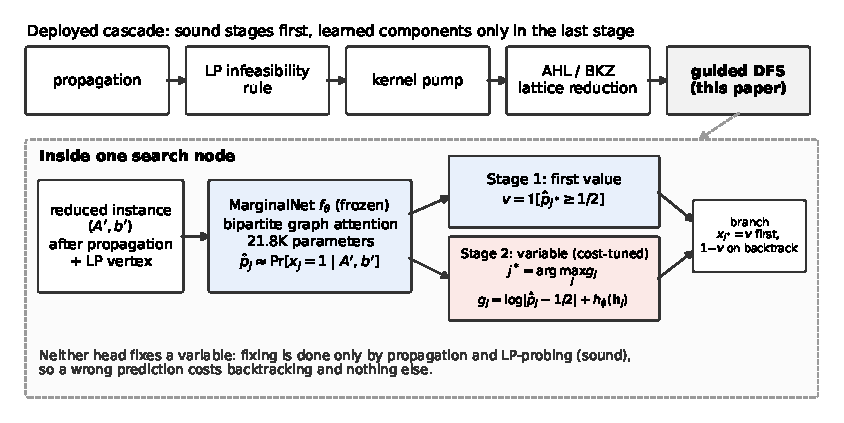
\includegraphics[width=\textwidth]{framework.pdf}
\caption{The deployed system and the two learned components. The cascade runs sound stages first; the learned components act only inside the final guided depth-first search. At a node, the frozen marginal network supplies $\hat p_j$; the value tried first comes from $\hat p$ (Stage~1), the variable branched on from the cost-tuned policy head (Stage~2). Neither fixes a variable.}
\label{fig:framework}
\end{figure*}

\subsection{Setting and search}
\label{sec:method-setting}

Given~\eqref{eq:bls}, a depth-first search maintains a partial assignment $\mathbf{x}_F=\mathbf{v}$ on a set $F$ of fixed variables and a set $K$ of free ones. At each node it runs unit propagation on the residual system, prunes if a row becomes unsatisfiable, and otherwise branches: it selects $j\in K$ and a first value $v$, explores $x_j=v$ first and $x_j=1-v$ on backtracking. Variables are ever \emph{fixed} only by sound deduction (propagation, and LP-probing where the opposite value makes the relaxation infeasible); the learned components decide the branching order and the first value, so a wrong prediction costs backtracking and nothing else. Figure~\ref{fig:framework} shows the deployed cascade: propagation, an LP-infeasibility rule, a kernel-pump heuristic and AHL/BKZ lattice reduction run first and close the easy part; the guided search sees the residual.

\subsection{Conditioning is reduction; which decisions cost anything}
\label{sec:method-reduce}

\begin{figure*}[t]
\centering
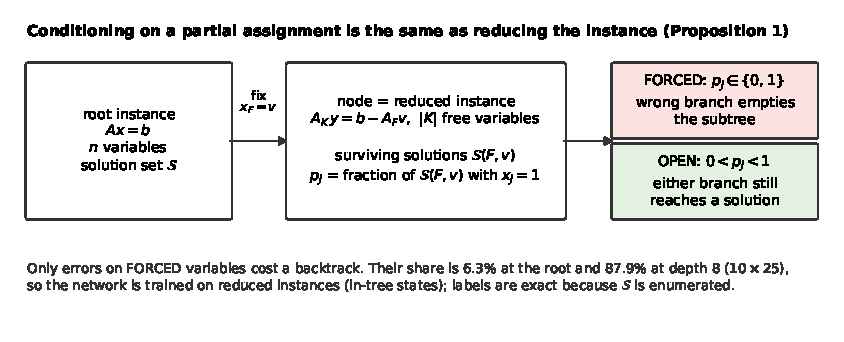
\includegraphics[width=\textwidth]{reduction.pdf}
\caption{Proposition~\ref{prop:reduce} and the partition it induces. A node with $\mathbf{x}_F=\mathbf{v}$ is the smaller BLS $A_K\mathbf{y}=\mathbf{b}-A_F\mathbf{v}$; its conditional marginals are the ordinary marginals of that instance. Variables on which every surviving solution agrees are $\FORCED$; only branching against them costs a backtrack.}
\label{fig:reduction}
\end{figure*}

Let $\SOL(F,\mathbf{v})=\{\mathbf{x}\in\SOL:\mathbf{x}_F=\mathbf{v}\}$ be the solutions consistent with the node and $p_j=\Pr[x_j{=}1\mid A,\mathbf{b},\mathbf{x}_F{=}\mathbf{v}]=|\{\mathbf{x}\in\SOL(F,\mathbf{v}):x_j{=}1\}|/|\SOL(F,\mathbf{v})|$ the conditional marginal, the posterior under the uniform prior on $\SOL$ that a planted-solution generator induces.

\begin{proposition}
\label{prop:reduce}
With $A_F,A_K$ the column submatrices indexed by $F,K$, the map $\mathbf{x}\mapsto\mathbf{x}_K$ is a bijection from $\SOL(F,\mathbf{v})$ onto $\{\mathbf{y}\in\{0,1\}^{|K|}:A_K\mathbf{y}=\mathbf{b}-A_F\mathbf{v}\}$. Hence the conditional marginals of the original instance are the ordinary marginals of the reduced instance.
\end{proposition}
\begin{proof}
$A\mathbf{x}=A_F\mathbf{x}_F+A_K\mathbf{x}_K$; with $\mathbf{x}_F=\mathbf{v}$ fixed, $A\mathbf{x}=\mathbf{b}$ iff $A_K\mathbf{x}_K=\mathbf{b}-A_F\mathbf{v}$, and $\mathbf{x}_F$ is determined, so the map is a bijection; the marginal statement follows by counting.
\end{proof}

Two consequences (Figure~\ref{fig:reduction}). First, one architecture, one label generator and one training loop serve every node: a depth-$d$ training state is stored as an instance on $n-d$ variables. Second, $p_j\in\{0,1\}$ means every surviving solution agrees on $x_j$; branching the other way empties the subtree. We call such variables $\FORCED$ and the rest $\FREE$: either branch of a $\FREE$ variable still reaches a solution, so a wrong first value there costs nothing beyond exploring a subtree that contains one. Only $\FORCED$ errors cost a backtrack. Their share grows as the search descends and $|\SOL(F,\mathbf{v})|$ shrinks --- $6.3\%$ at the root of a $10\times25$ instance, $87.9\%$ at depth $8$ (Section~\ref{sec:exp-pred}) --- which is why prediction is trained and evaluated inside the tree.

\subsection{Stage 1: exact conditional marginals as targets}
\label{sec:method-stage1}

\begin{figure*}[t]
\centering
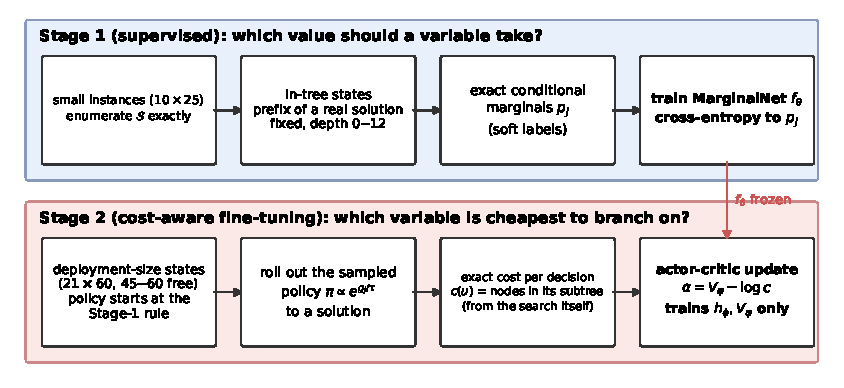
\includegraphics[width=\textwidth]{training.pdf}
\caption{The two training stages. Stage~1 learns \emph{which value} from exact conditional marginals of enumerable instances; Stage~2 learns \emph{which variable} from the exact subtree cost of every decision, produced by the search, with the Stage-1 network frozen.}
\label{fig:training}
\end{figure*}

On instances small enough to enumerate ($10\times25$ here), $\SOL$ is obtained with the all-solutions mode of a constraint solver and $p_j$ computed by counting. Only enumerations that run to exhaustion (\texttt{OPTIMAL} or \texttt{INFEASIBLE}) are accepted; a time-limited enumeration with solutions already collected would substitute a truncated $\SOL$ and bias every label. Training states are reachable in-tree states: a depth $d\in\{0,\dots,12\}$ is drawn uniformly, a prefix of an LP-confidence ordering is fixed to the values of a randomly chosen actual solution, and the reduced instance is enumerated in turn to give $p_j$ on its free variables. The network $f_\theta$ (MarginalNet) is a bipartite variable--constraint graph network with graph attention \citep{velickovic2018graph}: three features per variable node (its LP value, column density, fractionality), three per constraint node (right-hand side, row density, LP residual, each normalized by row size), hidden width $64$, four rounds of attention in each direction with residual connections and layer normalization, and one logit per variable; $21{,}761$ parameters. It is trained by cross-entropy against the soft targets $p_j$,
\begin{equation}
\mathcal{L}_1=-\tfrac{1}{|K|}\sum_{j\in K}\bigl[p_j\log\hat p_j+(1-p_j)\log(1-\hat p_j)\bigr],
\label{eq:loss1}
\end{equation}
minimized exactly at $\hat p=p$. Replacing $p_j$ by the planted solution, the usual choice, is a noisy surrogate whenever $|\SOL|>1$. At a node the network is evaluated once; the supervised branching rule is
\begin{equation}
j^\star=\arg\max_{j\in K}\,|\hat p_j-\tfrac12|,\qquad v=\mathbb{1}[\hat p_{j^\star}\ge\tfrac12].
\label{eq:rule1}
\end{equation}

\subsection{Stage 2: exact subtree costs as the objective}
\label{sec:method-stage2}

Rule~\eqref{eq:rule1} maximizes the chance that the first child contains a solution. It says nothing about how much the search pays when it does not, nor how much smaller the children are; both are properties of the subtree, and a depth-first search produces them exactly. Let $c(u)$ be the number of nodes expanded below node $u$ until a solution is found there or the subtree is exhausted; the search returns it when it backtracks out of $u$. Stage~2 fine-tunes the branching order on $-\log c(u)$.

\paragraph{Decision process.} A state is the reduced instance after propagation; an action is a free variable $j$; the first value stays $\mathbb{1}[\hat p_j\ge\frac12]$ from the frozen Stage-1 network. Because each decision owns its subtree, credit is assigned per decision rather than per episode --- the property that a sparse solved/unsolved reward lacks.

\paragraph{Policy and value.} On the frozen trunk of $f_\theta$ (variable embeddings $\mathbf{h}_j$) two heads are added. The policy logit is
\begin{equation}
g_j(s)=\log\bigl|\hat p_j-\tfrac12\bigr|+h_\phi(\mathbf{h}_j),
\label{eq:policy}
\end{equation}
with $h_\phi$ a two-layer network whose last layer is initialized to zero, so that $\pi(j\mid s)\propto\exp(g_j/\tau)$ starts as a softening of~\eqref{eq:rule1} and its argmax is exactly rule~\eqref{eq:rule1}. A value head $V_\psi(s)$ on a pooled graph embedding, $\log|K|$ and $\log m$ predicts $\log c$.

\paragraph{Update.} Each epoch samples training states, rolls the sampled policy ($\tau=1$) out to a solution, and records every decision with its cost. With the advantage $\alpha(u)=V_\psi(s_u)-\log c(u)$ standardized within the epoch,
\begin{equation}
\begin{split}
\mathcal{L}_2=\sum_u\Bigl[&-\alpha(u)\log\pi(j_u\mid s_u)-\lambda\,\mathcal{H}\bigl(\pi(\cdot\mid s_u)\bigr)\\
&+\bigl(V_\psi(s_u)-\log c(u)\bigr)^2\Bigr],\qquad\lambda=0.01.
\end{split}
\label{eq:loss2}
\end{equation}
Only $\phi,\psi$ are trained; $\theta$ is fixed, so the marginal that chooses values and defines the $\FORCED$/$\FREE$ partition is unchanged, and any improvement is attributable to the branching order alone. The critic is pre-trained on decisions recorded under rule~\eqref{eq:rule1}, and its held-out rank correlation with $\log c$ gates the actor update (a baseline that cannot rank costs makes the advantage noise). The epoch is selected on held-out states from the training pool, never on evaluation instances. At deployment the policy is greedy, $j^\star=\arg\max_j g_j(s)$ (Figure~\ref{fig:framework}).

\subsection{Cost per node}
\label{sec:method-cost}

At a node with $n_c$ free variables the network costs one relaxation plus one forward pass; LP-probing, the sound procedure that detects the same $\FORCED$ variables, costs $n_c$ relaxations. With a warm-started relaxation on both sides the measured ratio grows from $1.7\times$ at $n=25$ to $7.2\times$ at $n=60$ and $17.8\times$ at $n=150$, but is only $1.3$--$1.7\times$ at the depths where prediction matters on our instances, where probing additionally yields proofs. The Stage-2 head adds nothing measurable to the forward pass.

\section{Experiments}
\label{sec:exp}

\subsection{Instances and protocol}
\label{sec:exp-protocol}

Instances come from a market-split generator that plants a random $n/2$-of-$n$ solution and, among $20$ candidate plantings per $A$, keeps the one with the largest relaxation-vertex spread; no uniqueness is imposed. Solution multiplicity changes the task --- with $|\SOL|=1$ every variable is $\FORCED$ --- so $m$ is chosen per size to match it: $10\times25$ (median $|\SOL|=23$), $18\times50$ ($19$), $21\times60$ ($10$; $27/30$ verified). At $n=100$ a constraint solver finds no solution within $20$\,s, so search fails for every strategy and we stop at $n=60$. Stage~1 trains on $10{,}000$ in-tree states from $1{,}760$ instances at $10\times25$ (Adam, $10^{-3}$, $20$ epochs, batch $1$, gradient clipping $1.0$; $20$ minutes on one core); no hyperparameter was tuned and there is no validation split. Evaluation uses $30$ instances per size, plus a $100$-instance $21\times60$ set (generator seeds $700000$--$700099$, containing the thirty) built after the $30$-instance results were known. Stage~2 uses a separate $21\times60$ pool of $500$ instances (seeds $800000$+, $400/100$ split), whose overlap with every evaluation set is zero by hash of $(A,\mathbf{b})$; its $100$ held-out instances supply the states on which fine-tuning epochs are selected.

Every arm runs in the same loop: one warm-started relaxation per node (Gurobi dual simplex, bounds changed in place), identical propagation, identical value rule; arms differ only in the branching choice. Budgets are per-instance wall-clock, enforced by process termination; concurrency is $6$ on a $20$-core machine; all timing-sensitive code is single-threaded. Per-instance speed is tested with a two-sided sign test; node counts are seed-invariant because the search is deterministic given the relaxation vertex. Every $21\times60$ figure is replicated over three seeds. Enumeration and CP-SAT use OR-Tools; lattice reduction uses fpylll.

\subsection{Prediction against the exact posterior}
\label{sec:exp-pred}

\begin{table}[t]
\centering
\fitc{\begin{tabular}{lrrr}
\toprule
& root & depth 8 & all depths \\
\midrule
conditional Bayes ceiling & 70.8\% & 94.4\% & 87.2\% \\
MarginalNet (in-tree trained) & 66.7\% & 84.3\% & \textbf{80.0\%} \\
MarginalNet (root trained, controlled) & --- & 77.4\% & 75.4\% \\
LP relaxation rounding & 60.9\% & 80.9\% & 76.5\% \\
\midrule
$\FORCED$ share of variables & 6.3\% & 87.9\% & --- \\
\bottomrule
\end{tabular}}
\caption{Per-variable accuracy on held-out in-tree states of the $10\times25$ pool against the exact posterior. The controlled row trains on the same pool, labels, architecture and state count, on root states only.}
\label{tab:pred}
\end{table}

Table~\ref{tab:pred} places the Stage-1 network against the ceiling that no predictor can exceed, $\text{ceil}=\frac1{|K|}\sum_j\max(p_j,1-p_j)$. It closes most of the gap between relaxation rounding and the ceiling at every depth, and its $3$--$6$ point margin over rounding does not vanish deep in the tree. The composition, not the level, is what moves: the $\FORCED$ share rises from $6.3\%$ to $87.9\%$, so almost every decision at depth $8$ can cost a backtrack. Training on root states instead, with everything else controlled, gives a network that is \emph{worse} than rounding inside the tree ($75.4\%$ against $76.4\%$): in-tree supervision is what makes learned guidance better than the classical rule. A graph-free MLP on the same features reaches $79.4\%$ against the network's $84.1\%$ on a matched split, so the graph structure carries part of the margin. Where the margin lives at deployment size is shown in Figure~\ref{fig:results}c: inside the training range ($13$--$25$ free variables) network and rounding are indistinguishable (correlation $1.000$), because at constraint density $m/|K|\ge0.8$ the relaxation is already integral on every $\FORCED$ variable; the entire margin ($+5$ points) arises at $50$--$60$ free variables, outside the training range, where the relaxation is weakest ($m/|K|\approx0.35$--$0.42$). $80\%$ of the $21\times60$ search's queries fall there.

\subsection{Search performance}
\label{sec:exp-search}

\begin{table*}[t]
\centering
\fitw{\begin{tabular}{llrrrrl}
\toprule
size (budget) & strategy & solve rate & median nodes & median time & nodes/s & vs.\ previous row (per instance) \\
\midrule
$10\times25$ (60\,s) & \textsc{lp} & 100\% & 46 & $0.03$\,s & 1{,}767 & \\
 & \textsc{stage 1} & 100\% & 24 & $0.07$\,s & 376 & slower: forward pass exceeds a 24-node tree \\
\midrule
$18\times50$ (300\,s) & \textsc{lp} & 100\% & 4{,}224 & $2.43\pm0.33$\,s & 2{,}066 & \\
 & \textsc{stage 1} & 100\% & 1{,}085 & $1.82\pm0.37$\,s & 731 & $1.3$--$1.4\times$, $18/30$, n.s. \\
 & \textsc{stage 1+2} & 100\% & \textbf{424} & $\mathbf{0.52\pm0.01}$\,\textbf{s} & 820 & $1.8$--$2.2\times$, $22$--$24/30$, $p\le0.016$ \\
\midrule
$21\times60$, 30 inst.\ (600\,s) & \textsc{lp} & 100\% & 82{,}366 & $47.9\pm0.8$\,s & 1{,}627 & \\
 & \textsc{stage 1} & 100\% & 8{,}657 & $14.5\pm0.1$\,s & 619 & $2.6$--$3.0\times$, $23/30$, $p=0.005$ \\
 & \textsc{stage 1+2} (seed 0 / 1) & 100\% & 8{,}873 / \textbf{4{,}040} & $12.5$ / $\mathbf{5.9}$\,s & 710 / 690 & $1.2$--$1.5\times$ n.s.\ / $2.3\times$, $20$--$21/30$ \\
\midrule
$21\times60$, 100 inst.\ (600\,s) & \textsc{lp} & 100\% & 79{,}609 & $41.2\pm1.9$\,s & 1{,}966 & \\
 & \textsc{stage 1} & 100\% & 13{,}386 & $16.5\pm0.6$\,s & 796 & $2.0$--$2.3\times$, $70$--$71/100$, $p<0.001$ \\
 & \textsc{stage 1+2} (seed 0 / 1) & 100\% & 5{,}495 / \textbf{4{,}940} & $7.6$ / $\mathbf{6.8}$\,s & 738 / 730 & $2.0$--$2.2\times$ / $1.9$--$2.4\times$, $64$--$68/100$, $p\le0.007$ \\
\bottomrule
\end{tabular}}
\caption{Branching strategies in the same warm-started loop, lattice stage off, three seeds (mean $\pm$ s.d.\ of per-seed medians; node counts are seed-invariant). \textsc{lp} branches on the most integral relaxation value; \textsc{stage 1} is rule~\eqref{eq:rule1}; \textsc{stage 1+2} the cost-fine-tuned policy, trained at $21\times60$ only and reported for two training seeds. The last column compares each row with the row above it.}
\label{tab:search}
\end{table*}

Table~\ref{tab:search} is the main result. Three points. First, Stage~1 produces a smaller tree than the LP rule at every size ($2.0\times$, $3.9\times$, $5.5$--$9.5\times$ fewer nodes) and the ratio grows with size, as Figure~\ref{fig:results}c predicts; a smaller tree buys time only once the tree is large enough to pay for the forward pass, so at $10\times25$ Stage~1 is slower. Second, the $100$-instance set replicates the $21\times60$ result with power --- Stage~1 is faster on $70$--$71/100$ instances --- at smaller margins than the original thirty ($2.0$--$2.3\times$ against $2.6$--$3.0\times$), which are the first thirty seeds of the larger set and a favourable sample for Stage~1; we take the $100$-instance figures as the estimate. Third, Stage~2 removes a further $2.3$--$2.4\times$ of the nodes and $2.0$--$2.4\times$ of the time on $100$ instances, in both training seeds and every evaluation seed, at unchanged per-node cost, for $4.8$--$5.9\times$ over the LP rule end to end; the policy was fine-tuned at $21\times60$ only and transfers to $18\times50$ ($1.7\times$ fewer nodes, $1.8$--$2.2\times$ faster). On the original thirty the two training seeds differ (one is near Stage~1, one $1.9\times$ better), a spread the $100$-instance set does not show. Random branching, for reference, solves $0/30$ at $20\times50$ within $300$\,s and none of the $21\times60$ residual of Section~\ref{sec:exp-cascade}.

\begin{figure*}[t]
\centering
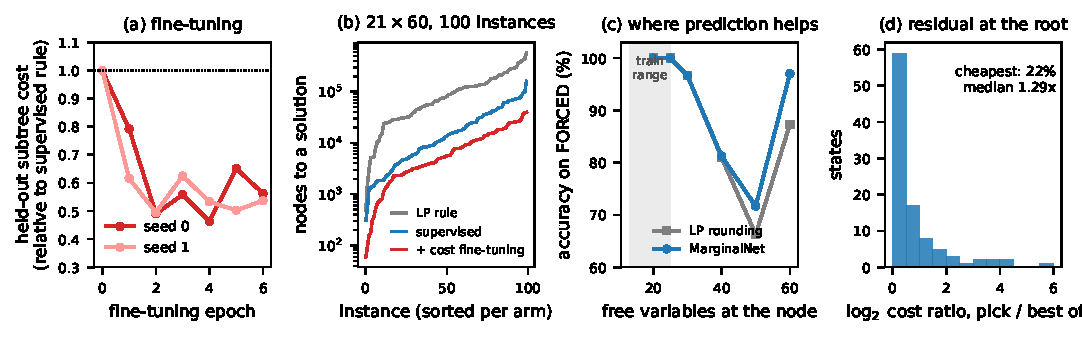
\includegraphics[width=\textwidth]{results.pdf}
\caption{(a) Stage-2 fine-tuning: total subtree cost on $150$ held-out states relative to the Stage-1 rule, two training seeds. (b) Nodes to a solution on the $100$-instance $21\times60$ set, each arm sorted. (c) Accuracy on $\FORCED$ variables of $21\times60$ in-tree states by number of free variables: the Stage-1 margin over relaxation rounding lies outside the training range. (d) Residual at the root: cost of the confidence rule's choice relative to the cheapest of its five candidates ($100$ held-out states, $45$--$50$ free variables).}
\label{fig:results}
\end{figure*}

\subsection{Against complete solvers}
\label{sec:exp-classical}

\begin{table}[t]
\centering
\fitc{\begin{tabular}{lrrrr}
\toprule
size & CP-SAT & SCIP & stage 1 & stage 1+2 \\
\midrule
$10\times25$ & \textbf{0.002\,s} & 0.009\,s & 0.07\,s & --- \\
$18\times50$ & \textbf{0.046\,s} & 0.385\,s & 1.82\,s & 0.52\,s \\
$21\times60$ (30) & \textbf{1.16\,s} & 3.69\,s & 14.5\,s & 5.9--12.5\,s \\
$21\times60$ (100) & \textbf{0.79\,s} & 2.59\,s & 16.5\,s & 6.8--7.6\,s \\
\bottomrule
\end{tabular}}
\caption{Median solve time, single-threaded, same instances and budgets; every method solves every instance. CP-SAT is $9$--$11\times$ faster than the full method at $21\times60$ and $11\times$ at $18\times50$.}
\label{tab:classical}
\end{table}

The method does not compete with a complete solver (Table~\ref{tab:classical}). The gap decomposes: at $21\times60$ CP-SAT's own branch counter reports a median of $18{,}827$ branches, more than our $4{,}040$--$8{,}873$ nodes, while it processes $19{,}782$ nodes/s against our $\sim\!700$ in Python, where the network's forward pass ($1.9$\,ms at the root) is now over $90\%$ of the per-node cost. The deficit is per-node throughput, not branching quality; whether it is recoverable with a compiled inference path and the clause learning and restarts our search lacks is not something we show.

\subsection{Deployment in the full pipeline}
\label{sec:exp-cascade}

\begin{table}[t]
\centering
\fitc{\begin{tabular}{llrrr}
\toprule
size & strategy & lattice & residual & time on residual \\
\midrule
$10\times25$ & any & 30/30 & --- & --- \\
$18\times50$ & \textsc{lp} / \textsc{stage 1} / \textsc{1+2} & 24--28/30 & 11/11 & 0.5--5.0 / 0.6--2.5 / 0.8--0.8\,s \\
$21\times60$ & random & 10--16/30 & \textbf{0/50} & $>600$\,s \\
$21\times60$ & \textsc{lp} & 10--16/30 & 50/50 & 52.9--65.1\,s \\
$21\times60$ & \textsc{stage 1} & 10--16/30 & 50/50 & 14.2--20.2\,s \\
$21\times60$ & \textsc{stage 1+2} & 10--16/30 & 50/50 & \textbf{7.3--11.7\,s} \\
\bottomrule
\end{tabular}}
\caption{Cascade with lattice reduction first, three seeds; lattice coverage varies with the seed's column permutations, and every arm within a seed receives the identical residual. Median time on the residual instances, range over seeds.}
\label{tab:cascade}
\end{table}

Lattice coverage falls with size ($30/30$, $24$--$28/30$, $10$--$16/30$), which is what leaves room for branching to matter. At $21\times60$ the residual is genuinely hard --- random branching closes none of the $50$ residual instances pooled over seeds --- and every sound strategy closes all of them; the difference is time. Stage~1 is $3.0\times$ faster than the LP rule on the residual ($40/50$, $p=2\times10^{-5}$) and Stage~2 a further $1.2$--$2.7\times$ depending on the seed's residual. End-to-end solve rate is $100\%$ for every sound arm and $44\%$ for random branching.

\subsection{Size transfer of Stage 1}
\label{sec:exp-transfer}

With $|\SOL|$ matched, a Stage-1 network trained only at $10\times25$ is not worse at $21\times60$ than one trained at $18\times50$: $8{,}657$ against $14{,}742$ median nodes, faster on $18$--$19/30$ instances (n.s.). Root accuracy holds its margin over rounding at $10\times25$, $20\times50$ and $40\times100$ ($+11.0$, $+7.2$, $+4.7$ points). This matters because exact labels exist only where enumeration completes; transfer lets a network trained there be deployed where they do not.

\subsection{What the supervised target misses}
\label{sec:exp-residual}

\paragraph{Aligning the training distribution does not help.} Figure~\ref{fig:results}c suggests an obvious fix: train Stage~1 where its margin lives. We built $2{,}691$ in-tree states with $30$--$60$ free variables from the $21\times60$ training pool (prefix of the LP ordering fixed to the planted solution; exact marginals; all states with $\le55$ free variables enumerate within $90$\,s, $291/400$ roots do) and trained the same architecture on them alone (\textsc{M1}) and on a half-and-half mix (\textsc{M2}). Accuracy on $\FORCED$ variables at $50$--$60$ free variables rises by about one point ($+6.1/+10.7$ against $+5.4/+9.7$ for Stage~1). The tree doubles: \textsc{M1} expands $21{,}337$ median nodes on the $100$-instance set against $13{,}386$ (fewer on $38/100$, $p=0.021$), \textsc{M2} $18{,}558$, and a switch that routes nodes with $\ge50$ free variables to \textsc{M1} recovers nothing ($17{,}252$). The reason is where the nodes are: two thirds of all decisions occur at $25$--$34$ free variables, and on such small dense states \textsc{M1}'s most confident variable is $\FORCED$-and-correct $77.6\%$ of the time against $94.4\%$ for Stage~1 (rank correlation with the true margin $0.12$ against $0.36$). A network slightly better at the top of the tree and much worse inside it makes the search slower. Within $10\times25$, training on depths $0$--$6$, $6$--$12$ or $0$--$12$ makes no difference ($79.3$/$79.9$/$79.9\%$). The training-state distribution is not the lever.

\paragraph{The confident choice is rarely the cheapest.} On $100$ held-out states with $45$--$50$ free variables we forced the root to each of the five most confident variables and ran rule~\eqref{eq:rule1} below. The rule's own choice is the cheapest of the five on $22\%$ of states; the median cost ratio to the best candidate is $1.29$, the mean $2.97$, a candidate at least twice as cheap exists on $24\%$ of states, and the best root choice alone would remove $55\%$ of the nodes summed over these states (Figure~\ref{fig:results}d). The residual is about \emph{which} variable, and it is large.

\subsection{Cost-aware fine-tuning}
\label{sec:exp-rl}

\paragraph{Critic gate.} Recording every decision of rule~\eqref{eq:rule1} on the training pool gives $37{,}275$ decisions ($9{,}375$ held-out) with exact subtree costs. The value head on the frozen trunk reaches a held-out Spearman correlation of $0.80$ with $\log c$; a baseline that knows only the state's size reaches $0.70$, and within size buckets the critic's advantage is larger ($0.68$ against $0.38$ at $35$--$44$ free variables). Unfreezing the trunk adds $0.02$; the frozen critic is used.

\paragraph{Fine-tuning.} Six epochs of $400$ rollouts from the $45$--$60$ free-variable training states ($\tau=1$, about $21{,}000$ decisions per epoch). Figure~\ref{fig:results}a shows the held-out monitor: total subtree cost falls to $0.46$ (seed $0$, epoch $4$ selected) and $0.50$ (seed $1$, epoch $2$) of the Stage-1 rule's, and policy entropy from $1.7$ to below $0.1$. The evaluation is in Table~\ref{tab:search} and Figure~\ref{fig:results}b.

\paragraph{What changed.} On $300$ held-out states the fine-tuned policy branches on a different root variable than rule~\eqref{eq:rule1} at $95\%$ of them; its pick is typically the $15$th most confident ($|\hat p-\frac12|$ of $0.26$ against $0.43$) and is $\FORCED$ with a correct first value less often ($57.5\%$ against $82.5\%$). The policy moved away from the variables the network is surest about, and the search got cheaper. The gain is not a property of the root decision alone: forcing only the root to the fine-tuned pick with rule~\eqref{eq:rule1} below gives a median cost ratio of $0.93$ (cheaper on $22/46$), so it is the sequence of decisions that improves. Two training seeds reach similar costs while choosing different variables at many nodes, as expected if the objective, not a particular solution, was learned. We can state what the fine-tuning optimizes but not yet name the feature it exploits; a cheap proxy, the propagation the first child triggers, does not differ between the two choices.

\section{Limitations}
\label{sec:limits}

\paragraph{Exact supervision bounds the method.} Marginals require enumerating $\SOL$, which does not complete beyond $n\approx60$; Stage~1 transfers to larger sizes but cannot be trained there, and Stage~2's cost signal, while available at any size the search runs at, was used at $21\times60$ only.

\paragraph{The useful size window is bounded on both sides.} Below it lattice reduction closes everything; above it ($n=100$) search fails for every strategy. Our demonstration lives at $n=50$--$60$.

\paragraph{The system is not competitive with CP-SAT} ($9$--$11\times$ slower), the deficit being per-node throughput in a Python loop dominated by the forward pass. Whether a compiled path plus clause learning closes it is not shown.

\paragraph{Statistical power and sampling.} The original thirty $21\times60$ instances proved a favourable sample for Stage~1 and an unstable one for Stage~2; the $100$-instance set is the estimate we stand behind, and Stage~2's cross-size transfer rests on thirty instances at $18\times50$.

\paragraph{Stage 2 rests on one training pool and two seeds.} Its entropy collapses within four epochs, the epoch is selected by a monitor rather than a stopping rule, and the feature it exploits is unnamed. No hyperparameter of either stage was tuned; the depth range of Stage~1 was subsequently shown not to matter within a size.

\paragraph{Single instance family.} Whether either signal transfers to other constraint families is untested.

\section{Conclusion}
\label{sec:conclusion}

A branching decision asks two questions, and we trained on an exact answer to each. The exact conditional posterior --- computable where solutions can be enumerated, and transported to every node by the reduction identity --- tells the search which value to try and identifies which predictions can cost anything; the exact subtree cost --- produced by the search as it backtracks --- tells it which variable to branch on. The first signal beats LP-guided branching by $2.0$--$2.3\times$ on $100$ hard $21\times60$ instances; the second, applied as a fine-tuning that leaves the first untouched, adds $2.0$--$2.4\times$, replicates across seeds and transfers down in size. That the fine-tuned policy prefers variables the posterior is less sure about, and that sharpening the posterior where its margin lives makes the tree larger, are the same fact seen twice: the probability of being right and the cost of being wrong are different objectives, and only the second is what a search minimizes.

\section*{Reproducibility}
Code is organized under \texttt{proposed\_src/} with a \texttt{ROLES.txt} per directory. Stage~1: \texttt{v15\_bayes/v15\_gen\_by\_m.py}, \texttt{v22\_transfer/v22\_split.py}, \texttt{v17\_conditional/v17\_make\_conditional\_data.py}, \texttt{v17\_train\_conditional.py}. Search and evaluation: \texttt{v23\_ablation/run\_revision2.sh}. Stage~2 and the residual experiments: \texttt{v24\_deploy\_range/run\_v24.sh}, \texttt{run\_v24\_r1.sh}, \texttt{run\_v24\_r2.sh}, \texttt{run\_v24\_r2b.sh}; figures: \texttt{make\_260917\_figures.py}. All generators are seeded; instance data and weights are regenerated rather than distributed.

\begin{thebibliography}{99}
\bibitem[Aardal et al.(2000a)]{aardal2000diophantine} Aardal, K., Hurkens, C. A. J., and Lenstra, A. K. (2000). Solving a system of linear Diophantine equations with lower and upper bounds on the variables. \emph{Mathematics of Operations Research}, 25(3):427--442.
\bibitem[Aardal et al.(2000b)]{aardal2000market} Aardal, K., Bixby, R. E., Hurkens, C. A. J., Lenstra, A. K., and Smeltink, J. W. (2000). Market split and basis reduction: Towards a solution of the Cornu\'ejols--Dawande instances. \emph{INFORMS Journal on Computing}, 12(3):192--202.
\bibitem[Amos(2023)]{amos2023tutorial} Amos, B. (2023). Tutorial on amortized optimization. \emph{Foundations and Trends in Machine Learning}, 16(5):592--732.
\bibitem[Chen et al.(2023)]{chen2023representing} Chen, Z., Liu, J., Wang, X., Lu, J., and Yin, W. (2023). On representing mixed-integer linear programs by graph neural networks. In \emph{International Conference on Learning Representations}.
\bibitem[Cornu\'ejols and Dawande(1999)]{cornuejols1999class} Cornu\'ejols, G. and Dawande, M. (1999). A class of hard small 0-1 programs. In \emph{Integer Programming and Combinatorial Optimization}, pages 284--293.
\bibitem[Etheve et al.(2020)]{etheve2020reinforcement} Etheve, M., Al\`es, Z., Bissuel, C., Juan, O., and Kedad-Sidhoum, S. (2020). Reinforcement learning for variable selection in a branch and bound algorithm. In \emph{CPAIOR}, pages 176--185.
\bibitem[Gasse et al.(2019)]{gasse2019exact} Gasse, M., Ch\'etelat, D., Ferroni, N., Charlin, L., and Lodi, A. (2019). Exact combinatorial optimization with graph convolutional neural networks. In \emph{Advances in Neural Information Processing Systems}, volume 32.
\bibitem[Gershman and Goodman(2014)]{gershman2014amortized} Gershman, S. J. and Goodman, N. D. (2014). Amortized inference in probabilistic reasoning. In \emph{Proceedings of the Annual Meeting of the Cognitive Science Society}, volume 36.
\bibitem[Haralick and Elliott(1980)]{haralick1980increasing} Haralick, R. M. and Elliott, G. L. (1980). Increasing tree search efficiency for constraint satisfaction problems. \emph{Artificial Intelligence}, 14(3):263--313.
\bibitem[Khalil et al.(2016)]{khalil2016learning} Khalil, E. B., Le Bodic, P., Song, L., Nemhauser, G., and Dilkina, B. (2016). Learning to branch in mixed integer programming. In \emph{AAAI Conference on Artificial Intelligence}.
\bibitem[Lenstra et al.(1982)]{lenstra1982factoring} Lenstra, A. K., Lenstra, H. W., and Lov\'asz, L. (1982). Factoring polynomials with rational coefficients. \emph{Mathematische Annalen}, 261(4):515--534.
\bibitem[Li et al.(2023)]{li2023g4satbench} Li, Z., Guo, J., and Si, X. (2023). G4SATBench: Benchmarking and advancing SAT solving with graph neural networks. \emph{Transactions on Machine Learning Research}.
\bibitem[Marques-Silva and Sakallah(1999)]{marquessilva1999grasp} Marques-Silva, J. P. and Sakallah, K. A. (1999). GRASP: A search algorithm for propositional satisfiability. \emph{IEEE Transactions on Computers}, 48(5):506--521.
\bibitem[Ohrimenko et al.(2009)]{ohrimenko2009propagation} Ohrimenko, O., Stuckey, P. J., and Codish, M. (2009). Propagation via lazy clause generation. \emph{Constraints}, 14(3):357--391.
\bibitem[Scavuzzo et al.(2022)]{scavuzzo2022learning} Scavuzzo, L., Chen, F. Y., Ch\'etelat, D., Gasse, M., Lodi, A., Yorke-Smith, N., and Aardal, K. (2022). Learning to branch with tree MDPs. In \emph{Advances in Neural Information Processing Systems}, volume 35.
\bibitem[Schnorr and Euchner(1994)]{schnorr1994lattice} Schnorr, C. P. and Euchner, M. (1994). Lattice basis reduction: Improved practical algorithms and solving subset sum problems. \emph{Mathematical Programming}, 66:181--199.
\bibitem[Selsam et al.(2019)]{selsam2019neurosat} Selsam, D., Lamm, M., B\"unz, B., Liang, P., de Moura, L., and Dill, D. L. (2019). Learning a SAT solver from single-bit supervision. In \emph{International Conference on Learning Representations}.
\bibitem[Veli\v{c}kovi\'c et al.(2018)]{velickovic2018graph} Veli\v{c}kovi\'c, P., Cucurull, G., Casanova, A., Romero, A., Li\`o, P., and Bengio, Y. (2018). Graph attention networks. In \emph{International Conference on Learning Representations}.
\bibitem[Williams(1992)]{williams1992simple} Williams, R. J. (1992). Simple statistical gradient-following algorithms for connectionist reinforcement learning. \emph{Machine Learning}, 8(3--4):229--256.
\end{thebibliography}
\end{document}
